% This file should be replaced with your file with an thesis content.
%=========================================================================
% Authors: Michal Bidlo, Bohuslav Křena, Jaroslav Dytrych, Petr Veigend and Adam Herout 2019

\chapter{Introduction}
importance of GUI testing, goals, regressions, errors 

The goal of this work is to design and implement a tool for generating tests for GNOME desktop applications using AT-SPI metadata created as a by-product of an architecture supporting assistive technologies.

The architecture expose application as a tree of accessibility objects with their current state. Every object is defined by several properties and set of actions that can be invoked to change the current state. Since accessibility support has been implemented to very fundamental layers of GTK/GNOME framework (widget level), it provides a suitable way for development of automated test suites.\cite{pyatspi2} 

Modern GUI applications are being developed more rapidly with lack of proper regression testing. 

manual testing vs automation clanok

Additionally this effort should also help to reveal defects and missing parts in accessibility itself and improve the experience for users with disabilities.

\chapter{Accessibility}
Accessibility in general is a technology that helps people with disabilities to participate in essential life activities. Considering the accessibility as a part of GNOME desktop, it includes libraries and development tools allowing users with disabilities to use other options of interaction with GNOME desktop environment. Those options includes voice interfaces, screen readers and other alternative input devices.\cite{gnomeADG}
\section{The Accessibility Toolkit (ATK)}
Assistive technologies are receiving information from the Accessibility toolkit (ATK), which offers built-in APIs for all GNOME widgets. ATK provides a set of interfaces which are required to be implemented by GUI components. Therefore, assistive technologies are able to automatically read most of the labels on screen without any extra efforts made by developers. The interfaces are toolkit-independent, meaning that their implementation could be written for many widgets, including widgets from frameworks such as GTK\footnote{https://www.gtk.org/} and Qt\footnote{https://www.qt.io/}.
\section{GNOME Accessibility Implementation Library (GAIL)}
Majority of GNOME applications are written in GTK framework. The framework provides dynamically loadable module named GAIL implementing ATK interfaces for all GTK widgets. Once the module is loaded at runtime, the application is fully capable to cooperate with ATK without any further modifications.
GNOME desktop does not load accessibility support libraries by default, it has to be enabled by setting a special gsettings key, which can be achieved either by dconf\footnote{https://wiki.gnome.org/Projects/dconf} editor or via \texttt{gsettings} command line utility using a terminal application:
\begin{verbatim}
    gsettings get org.gnome.desktop.interface toolkit-accessibility true
\end{verbatim}
Additional configurations may be required for applications written in other frameworks such as QT or Java. Furthermore, implementations of other assitive technologies might be too application specific or use various techniques like OS event snooping etc. Compared to GNOME Desktop, all information required by assistive technologies (AT) are passed from GNOME Accessibility Framework to a toolkit-independent Service Provider Interface (SPI). The SPI is a key component providing stable and consistent API for screen readers, magnifiers, etc. Accessibility support is relying on per-toolkit implementation (GTK, QT, Java) and its APIs exported through relevant bridges to unified AT-SPI interface as described on Diagram \ref{ATSPI_architecture}.

\begin{figure}[hbt]
	\centering
	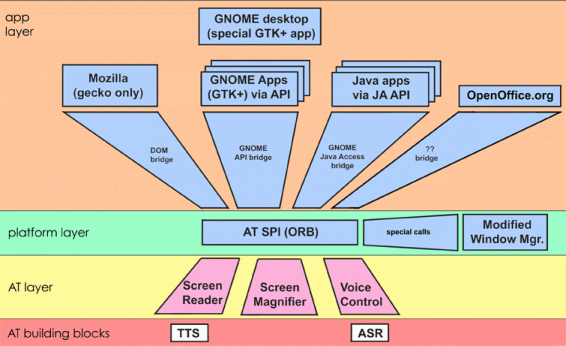
\includegraphics[width=1\textwidth]{obrazky-figures/GNOME_desktop_Accessibility.png}
	\caption{GNOME Accessibility Architecture overview}
	\label{ATSPI_architecture}
\end{figure}

The widget is accessible, if a developer uses any GTK/GNOME widget and follows the general accessibility guidelines\footnote{https://developer.gnome.org/accessibility-devel-guide/stable/gad-coding-guidelines.html.en} with properly implemented ATK interfaces. Considering that the stock GTK/GNOME toolkit widgets have implementations of these interfaces provided, new widgets will inherit the functionality and gain suitable accessibility support as well. The default implementation of ATK interfaces might be altered by applications, as developers can enrich their descriptions of widgets and improve the overall user experience in special cases, e.g. when widget is used for some less expected purposes or the default description is too general. The ATK provides set of functions to achieve this along with the ability to make any custom component accessible\footnote{https://developer.gnome.org/accessibility-devel-guide/stable/gad-custom.html.en}.\cite{accessibleWidgets}

\newpage
\section{Library pyatspi}
Package pyataspi is a Python wrapper around AT-SPI's C implementation, which loads the Accessibility typelib and imports the classes implementing AT-SPI interfaces.\cite{pyatspi}

AT-SPI exposes applications as a tree of widgets, starting with a root element where every sub-element represent one running application on the GNOME desktop. Each application has zero or more child elements, each child is distinguishable by its position in the tree and several object properties. Some of these properties are encapsulated inside the accessible object and their values must be obtained through corresponding methods, so called getters. Small set of properties are described in the following list:
\begin{itemize}
    \item \textit{name} - string value, for most widgets contains text identical with a text label visible on widget
    \item \textit{roleName} - string value, specifies the widget type, available via \textit{getRoleName} method
    \item \textit{childCount} - integer value, a number of sub-elements 
    \item \textit{actions} - list of strings, contains available actions which can be performed by the ATK
    \item \textit{visible} - boolean value, indicated that object is visible to the user
    \item \textit{showing} - boolean value, object is rendered
    \item \textit{text} - string value, mostly used in input fields or widgets containing plenty of text
    \item \textit{description} - string value, contains special widget description for users
    \item \textit{position} - integer tuple, x, y coordinates on the screen (might be related to other component)
    \item \textit{size} - integer tuple, shows height and width of a widget
\end{itemize}

Additionally, elements can be linked together in other useful ways (except parent-child relationship) where labels are linked with widgets like text fields, check boxes, combo boxes etc. These labels are making widgets easier to find or interact with. Other advantageous properties like \textit{showing} or \textit{visible} can be used to decide whether elements are hidden from the active screen area, thus they are not available for interaction. Specifying a \textit{roleName} allows categorization of widgets which is useful for identification of category specific methods, e.g. selecting values in radio buttons, selecting options in combo boxes or a simple click method on push buttons. Access to this functionality is focused in a singleton object named \textit{registry} that provides services for subscribing to specific events and generating events from mouse or keyboard on demand.

Library pyatspi is an open source project available for most of Linux distributions via distro specific packaging services (package named \textit{python3-atspi}) or is available to be built from its sources\footnote{https://gitlab.gnome.org/GNOME/pyatspi2}.

\section{Exploring and Debugging the Accesibility}
Currently, there are several tools available for exploration and debugging accessibility features not only on GNOME desktop. 
\subsection{Library dogtail}
Dogtail is an open source GUI test framework written in Python implemented as a library around pyatspi. Several modules implements higher level of API to simplify work and interaction with accessible objects during test development. The tool offers less complex functionality, containing tree view of objects with their basic attributes\cite{dogtail_doc}. Dogtail package also includes a GUI tool Sniff, similar to the Accerciser application described in the next section. The most important dogtail modules are described in several next paragraphs.

The module \textit{tree} contains the most important class \textit{Node}, instances of the class represent elements of the desktop user interface. All elements are gathered to tree structure, representing all applications starting with the root element (desktop). The class is implemented as a mixin for Accessible and various Accessible interfaces and is an important unit for it's subclasses, namely \textit{Application}, \textit{Root} and \textit{Window}. The Node class also implements methods used for search of nodes in the tree based on certain criteria. A lambda expression can be passed to methods \textit{findChild} and \textit{findChildren} as argument named \textit{pred}. The lambda expression can contain any properties that uniquely identify nodes, including \textit{name}, \textit{roleName},  \textit{showing} and \textit{visible}. The class also contains action methods that can be performed on nodes without importing other action modules. Verification and identification of shown nodes are easier thanks to method named \textit{blink}. Once the method is called on a certain element, the element is highlighted on the screen for several seconds. This functionality is also part of the Sniff tool where element is highlighted after it is selected in the displayed tree.

The module \textit{dump} contains only one method with the same name, the method return a string describing the tree of nodes which is useful for python/ipython console debugging.

Finally, the module \textit{rawinput} contains implementation required for generating events from both keyboard and mouse. More complex events simulating keyboard shortcuts, mouse gestures and drag and drop operations are implemented as well.  


 \begin{figure}[hbt]
	\centering
	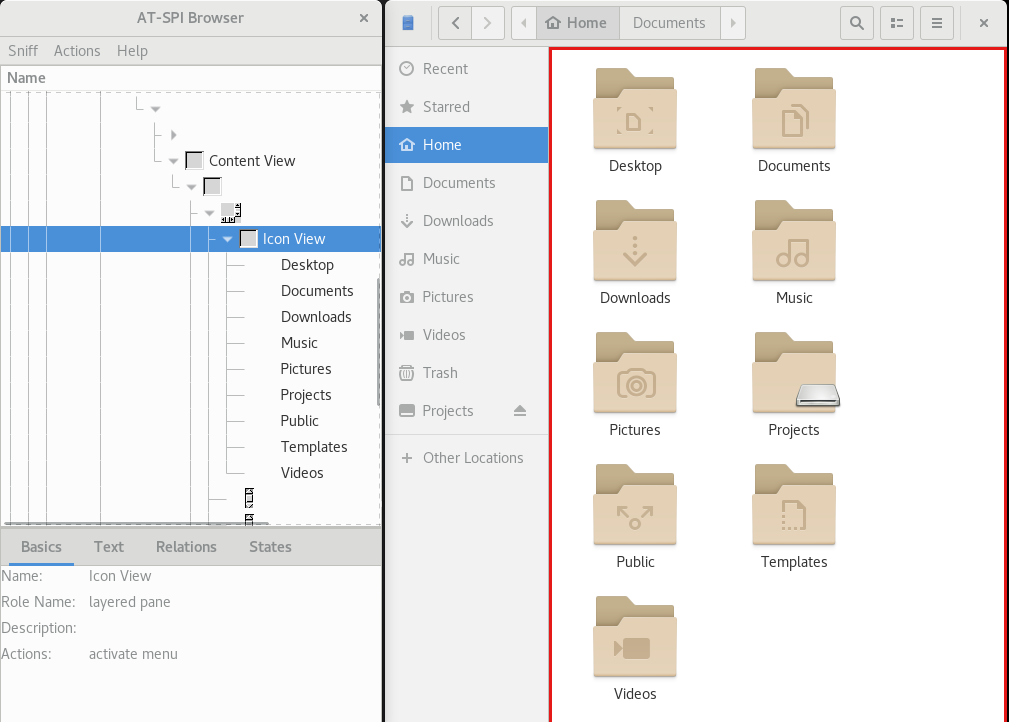
\includegraphics[width=1\textwidth]{obrazky-figures/sniff.png}
	\caption{Sniff utility highlighting icon area in Nautilus File Manager, Screenshot taken from Red Hat Enterprise Linux 8.2}
	\label{sniff}
\end{figure}

 Testing Dogtail has proven availability for many Linux distributions through their package repositories, specifically Fedora 32, Red Hat Enterprise Linux 8.2 and Manjaro 18 with GNOME 3.34 (Archlinux). It is also available as a Pypi Python package and according to information in it's official Gitlab repository should work not only for GTK+ application but also for application written in QT and KDE. 
 
 Dogtail testing reveals also some minor problems which might occur during the test development. To be more specific, there are know cases in which the coordinates of a node were not reported correctly. Most of the items labelled with a \textit{roleName} panel and list list box are missing their \textit{name} labels. Those items are not as important for users as they don't contain any visible text, nor an action to interact with. The purpose of those items is to serve as a wrapper for other elements and group them together in an element tree. Further testing discovered non-accessible menu\footnote{https://bugzilla.redhat.com/show_bug.cgi?id=1723836} or nameless menu button\footnote{https://wiki.gnome.org/Apps/DiskUsageAnalyzer}. So once an action needs to be dispatched on such element, the identification has to be done either through a parent element or a sibling element. Additionally, execution of a mouse event will require an offset calculation to specify the correct element position on the screen.
 
 So to conclude this chapter, dogtail is powerful tool for development of automated test cases in GNOME 3 environment. On the other hand, it contains discussed limitations and flaws. Those limitations mustn't come from the dogtail itself, they are either accessibility bugs or bugs in GTK framework (non-accessible menu).  

\subsection{Accerciser}
Accerciser is an interactive accessibility explorer developed in Python. It provides well-arranged graphical frontend for AT-SPI library, hence it can inspect, examine and interact with widgets and also allows developers to verify that their applications are providing correct information to assistive technologies and automated testing frameworks. The default interface has three sections: A tree view with the entire desktop accessible hierarchy and two optional plugin areas. Accerciser has an extensible, plugin-based architecture, most of the features available by default are provided by plugins discussed in next several paragraphs.

The Interface Viewer plugin is an explorer of AT-SPI interfaces provided by each accessible widget of a target application. Once an item is selected, its interfaces are shown with a list of sensitive methods, so all methods are executable. The list contains methods for interaction with an object and various methods for obtaining more information about the object. Accerciser allows to explore the following interfaces:
    \begin{itemize}
        \item Accessible - shows child count (number of child widgets), description, states, relations and other attributes
        \item Application - if implemented (not mandatory), it shows application ID, toolkit and version
        \item Component - shows item's absolute position with respect to the desktop coordinate system, relative position with respect to the  window coordinate system, size, layer type, MDI-Z-order indicating the stacking order of the component and alpha
        \item Document - shows document attributes and locale information
        \item Hypertext - shows a list with all item's hypertext links,  including name, URI, start index and end index
        \item Image - shows item's description, size, position and locale
        \item Selection - shows all selectable child items of the selected item,
        \item Streamable Content - shows selected item's content type and their corresponding URIs
        \item Table - shows item's caption, rows, columns, number of selected rows, number of selected columns and for selected cell, it shows  it's row's and column's header extents  
        \item Text - shows selected item's text content, that can be editable with attributes offset, justification  and possibility to show CSS formatting as well
        \item Value shows item's value, minimum value, maximum value, minimal increment for a value 
    \end{itemize}
    
The AT-SPI Validator plugin applies tests to verify the accessibility of a target application, the validator will generate the report of the selected item and all its descendant widgets in the tree hierarchy.

The next plugin is the Event Monitor, which displays AT-SPI emitted events including the filter for several different AT-SPI event classes. The plugin has the ability to monitor only events sourced from selected application or selected accessible (widget). Each event record contains the source and the application.

The Quict Select plugin provides global hotkeys for quickly selecting accessible widgets in Accerciser's Application Tree View, selected widget is highlighted in the target application.

The API Browser plugin shows interfaces, methods and attributes available on each accessible widgets of a target application, by default it shows only public methods and properties, private methods and properties are hidden until checkbox \textit{Hide Private Attributes} is unchecked.
 
Finally, plugin IPython Console provides full, interactive Python shell with access to selected accessible widgets of a target application as an pyatspi objects. Any object selected in the the tree view is available in the IPython Console under the symbol \textit{acc}, so the plugin provides an easy way to test and debug code used in test cases.    

\begin{figure}[hbt]
	\centering
	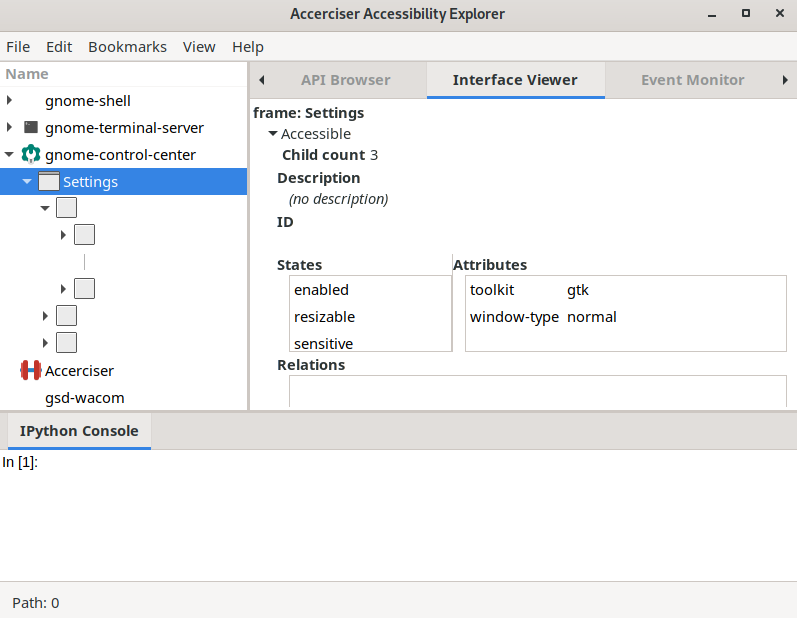
\includegraphics[width=1\textwidth]{obrazky-figures/accerciser.png}
	\caption{Accerciser default configuration, Screenshot taken on Manjaro Linux with GNOME 3.34}
	\label{Accerciser}
\end{figure}


\section{Covering Limitations of Accessibility and Verification}
As discussed in aforementioned sections information provided by accessibility is not flawless, therefore next couple chapters are dedicated to exploration of technologies that might be used to support the accessibility in such cases.

\subsection{OpenCV and Image Matching Techniques}
OpenCV or Open Source Computer Vision Library is a software library that provides optimized algorithms for computer vision and machine learning. According to official OpenCV webpage\cite{opencv}, the library contains more then 2500 algorithms and it is being developed 
by a vast community of contributors around the world. The library is used extensively bu government institutions, research groups and companies including Microsoft, Google, IBM and many more. One of the biggest advantages is its native C++ implementation with bindings making the library available in Python, Java and Matlab and supports Linux, Android, Mac OSX and Windows. Regardless of Linux distribution, similarly to dogtail, OpenCV can be installed easily via python3 package manager(pip). 

From the rich availability of algorithms provided, the image recognition algorithm can be used to either locate or verify the presence of an element on the screen. This approach would require to have set of images containing elements prepared in advance, then it can be used to find the image location on the screenshot of the screen taken during a test run. Compared to verification of the node only via accessibility, this approach would also verify that the element is properly rendering on screen and the shown result is really an element that is shown to the user. Additional benefit is verification of text formatting and colors. On contrary, there this process requires additional manual work of taking images, labelling them and associating them with certain test scenarios. Count of elements displayed on the screen multiple times creates another parameter which would require manual maintenance. The most common example of such case are buttons labelled either OK or Cancel as they are used in many applications.

Another possible approach is to use the shape recognition algorithm which can locate shapes like circles, rectangles and many other common shapes. From the development perspective this would be easier to maintain as there is no requirement for images prepared in advance. It can also help with the widget location in cases where accessibility is reporting wrong coordinates. On the other hand, locating the right widget in cases when several similarly shaped ones are located on the screen at the same time will yield very inconsistent results.


\subsection{OCR}
Optical Character Recognition or OCR is a method of extracting text from images. One of available open source tools is a tool called Tesseract.

Initially, Tesseract development started in 1985 at Hewlet Packard Laboratories but the major breakthrough was achieved in 2006 when the project was open sourced in cooperation with University of Nevada in Las Vegas. Since then, the project has been developed under the sponsorship of Google\cite{tesseract_history}.

Usability of Tesseract was increased in version 3.x, supporting wide range of image formats and gaining ability to be used in larger number of scripting languages. While Tesseract 3.x is based on traditional computer vision algorithms, in the past few years methods based on Deep Learning have surpassed traditional machine learning techniques by a vast margin, especially in terms of accuracy in several areas of Computer Vision. Remarkable results were achieved in handwriting recognition. Tesseract has implemented a Long Short Term Memory(LTSM) based recognition engine which is a kind of Recurrent Neural Network(RNN). While this kind of RNN is used for to recognize text of random length, a Convolutional Neural Network is used just for recognition of single character. Version 4 provides both legacy OCR engine and new LSTM engine which is enabled by default.\cite{tesseract}

Tesseract can be used as a command line tool, integration in development is possible via Tesseract's API available in python or C++. Setup on Linux or other platforms may differ but the process is accurately described in Tesseract's wiki\footnote{https://github.com/tesseract-ocr/tesseract/wiki}, with the last resort solution - building it from its sources.
The setup process includes installation of tesseract-ocr package itself, pytesseract python bindings installable via python's package manager pip and Tesseract's language pack with trained data for English language(version 4.x supports 130 languages\footnote{https://github.com/tesseract-ocr/tesseract/wiki/Data-Files#data-files-for-version-400-november-29-2016}). 

Tesseract's OCR engine works best when used with images containing black text on white background in a common font. Text should be approximately horizontal with the height of at least 20 pixels. Surrounding borders around the text can be detected as some random text. With possibilities of image processing provided by OpenCV, the image quality in some cases needs to be improved before applying text detection methods. Most common image preprocessing methods include inverting images, rescaling, binarisation, noise removal, rotation, border removal and page segmentation\footnote{https://github.com/tesseract-ocr/tesseract/wiki/ImproveQuality}.

Tesseract's API for python is bundled in a module named \texttt{pytesseract}. The module provides several methods, the most important ones for the purposes of this work are \verb|image_to_string| and \verb|image_to_data|. Both methods have one compulsory parameter which is an image intended for text extraction. An image has to be in certain format, one of the options is to load the image through OpenCV's \texttt{imread} method. Additional parameters may be applied including language, timeout and engine configuration\footnote{https://pypi.org/project/pytesseract/}. The first method returns all recognized strings including all whitespaces and other special characters. The second method provides additional metadata about all recognized strings in a form of dictionary like object. The returned dictionary contains the following lists of properties:

\begin{itemize}
    \item text - string value, may contain string, special character, one word or line of text
    \item left - integer value, specifies number of pixels from the left side of the image 
    \item top - integer value, specifies number of pixels from the top of the image
    \item width - integer value, specifies width of the recognized string 
    \item height - integer value, specifies height of the recognized string
    \item the rest are less important values for this work: \verb|level, page_num, block_num par_num|
    \verb| line_num, word_num, conf|
\end{itemize}

Therefore, occurrences of certain string in an image are filtered and highlighted in every image as demonstrated on Figure \ref{ocr_nautilus} for string \textit{Documents}.

\begin{figure}[hbt]
	\centering
	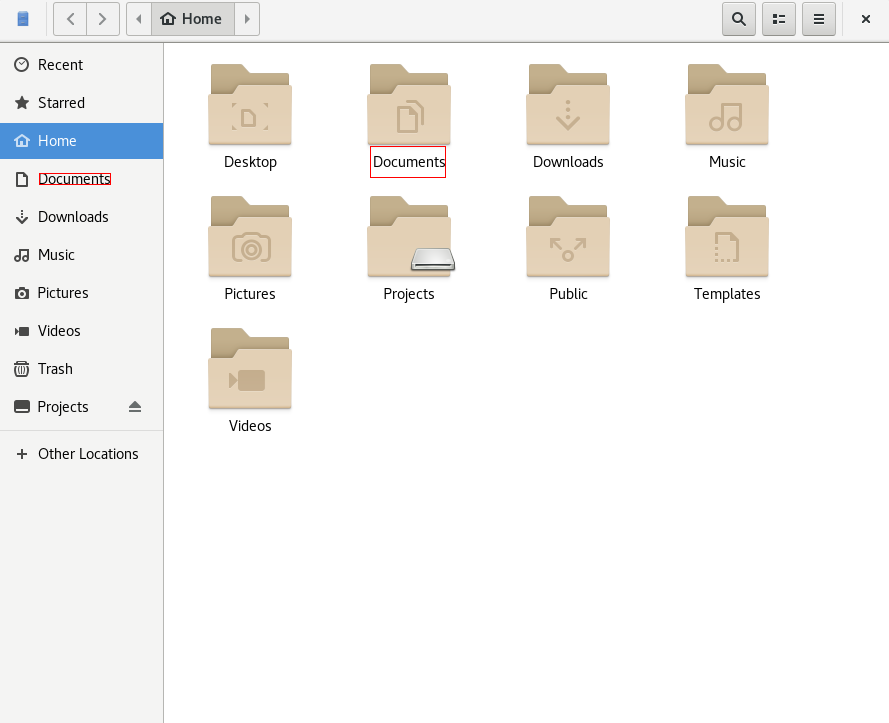
\includegraphics[width=1\textwidth]{obrazky-figures/ocr+nautilus.png}
	\caption{Demonstration of the OCR engine detection for the string Documents in Nautilus File Manager window, Red Hat Enterprise Linux 8.2}
	\label{ocr_nautilus}
\end{figure}

Similarly to OpenCV, Tesseract's OCR engine was tested as an alternative tool for location or verification of widgets which contain text. This method also verifies that the content was properly rendered and is readable for user. OCR systems have limitations and work with certain margin of error which is a fact that also applies to Tesseract. Various applications can use different color schemes including background colors and font colors, input fields and labels. Highlighting elements to perform actions on them can also lead to changes of these conditions. Image preprocessing methods provided by OpenCV can aid to avoiding problems associated with those cases, namely color inversion and binarisation. Those methods would supply Tesseract's engine with an image containing black text and white background for evaluation.

\section{Conclusion}
This chapter has been dedicated to the Accessibility technologies in GNOME desktop with a deeper look on implementation, libraries and tools for debugging. Furthermore, technologies that may be able to cover limitations and bugs in accessibility has been evaluated as well. Both OpenCV and Tesseract may help with identification, location and verification of non-accessible elements in applications. Possible disadvantage is a delay caused by taking and processing screenshots of applications that have to be taken on the right time. OpenCV's image matching algorithm can reliably locate prearranged images of icons, labels or whole application windows on the screen. Considering the stable application environment with black text on white background in most of applications, Tesseract is able to detect and reliably locate most of the text content on the screen. Other cases can be covered by image preprocessing done again in OpenCV. Furthermore, both technologies are working with actual application content rendered to users, possibly bringing additional level of verification.

\chapter{Testing Graphical User Interfaces}
Graphical user interfaces (GUI) is an interface that makes advantage of the computer's graphics capabilities to make software easier to use.\cite{guidefinition} Graphical applications are developed using sets of windows and widgets. A widget represents a graphical element describing certain behaviour and functionality. GUIs are able to perform tasks through events in different ways. Despite the fact that they improve usability and flexibility, they also represent a challenge for software testing and testers have to decide whether to check all event sequences of events or only a subset. The effort required to to test the GUIs can be reduced with automated software testing. Even though there were the significant progress made in automated testing tools over last decade, manual testing is still the most common technique in practice. However, with a proper automated GUI testing process, more test cases can be executed regularly and more faults can be found within less time.
\cite{patternbasedtesting}

Next several chapter are dedicated to various testing techniques with examples of tools using them. 

% \section{Testing Techniques Overview}


\section{Random Input Testing}
This testing technique is also referred as stochastic testing or monkey testing. The term monkey is mentioned in any form of automated testing performed without any user bias. This method distinguishes 3 types of monkeys testing the application by generating random sequences of events from keyboard and mouse. Dumb monkeys do not have any knowledge about the system, nor its state and they are not aware which actions are legal or illegal. The downsize is that they cannot recognize a failure when they encounter one. Their only goal is to crash the system under the test. Other group, referred as semismart monkeys, can recognize a bug when they see one. The last group are smart monkeys who have certain knowledge about the application they are testing, obtained from a state table or a model of system under test. On the other hand smart monkeys are the most expensive to develop. Despite the fact that random testing tool have a weak coverage, Microsoft has reported that 10-20\% in their software were discovered by random input testing method.\cite{nyman}

\section{Manual Testing}
In general, high-level Graphical User Interface (GUI) and acceptance tests are being performed manually. Those practices are often inefficient, error prone and tedious, especially when tests are pushed and executed in a hurry during late development stages. Manual tests are often pre-defined sets of steps performed on high level of system abstraction to validate system against required specification. However, a software is prone to changes and therefore the software needs to be tested against regressions. This leads to an excessive costs, since testers have to continuously re-execute test plans.\cite{guitesting}

\section{Record and Replay Tools}
To mitigate mentioned concerns and increase the end quality of software, an automated testing has been proposed as a solution. Considerable amount of work has been devoted to high-level test automation, resulting in Record and Replay techniques. Tool record the coordinates and properties of GUI components during manual user interaction. Obtained recording are being played back to emulate user interaction and validate the correct state of system during the regression testing. These techniques have also certain limitations, which are typically sensitivity to GUI layout changes and code changes. Therefore, obtained recording are not applicable, with additional costs of maintaining the tests.\cite{guitesting}

Example of this category of tools is the open source project GNU Xnee. The project consist from libraries and two applications. Test automation is one of the several use cases for this project. However the project is limited to X11 environments.\cite{xnee}

\section{Solutions Based on Image Recognition}
Visual GUI testing is an emerging technique combining scripting with image recognition, examples are open source tool Sikuli and commercial tool JAutomate. Image recognition allows to tests various systems regardless of their implementation, operating systems or even platform. Image recognition provides support for emulating user interaction with the bitmap components (images, buttons) shown to a user on the screen. However, the solutions based on image recognition are not suitable to be used with highly animated GUIs.\cite{guitesting}

Trivial automation of GUIs via image matching algorithm can be achieved with a Python module named Xpresser. The tool works with a directory of images containing cropped images of widgets. Image matching algorithms are used to identify the location of cropped images on screen and then perform an action. Xpresser is mostly used for testing on Ubuntu Linux distribution.\cite{xpresser}

\chapter{Proposed solution}
\section{Model extraction from accessibility}
\section{Test generation}
\section{Test case management}
behave - git
\section{Test case execution and reports}
\section{AppStream data}

\chapter{Conclusion}